\newcommand{\myFontSize}[0] {10pt}
\newcommand{\mySpacing}[0] {1.3}

\newcommand{\thesisTitle}[0] {Evaluating Recommender Systems for Digital Library Datasets}
%Odporúčacie systémy založené na AI
\documentclass[\myFontSize,oneside,english,hidelinks,a4paper]{article} 
%%%%%%%%%%%%%%%%%%%%%%%%%%%%%%%%%%%%%%%%%%%%%%%%%%%
\usepackage{graphicx}
\usepackage{float}
\usepackage{longtable}
\usepackage{setspace}
\usepackage{url} 
\usepackage{doi} 
\usepackage{cite}
\usepackage{comment} 
\usepackage[utf8]{inputenc}
\usepackage{enumitem}
\usepackage{titlesec}
\usepackage{multicol}
\usepackage{hyperref}
\usepackage[a4paper, top=0.8in, bottom=0.8in, left=0.8in, right=0.8in]{geometry}
\usepackage[parfill]{parskip}
\usepackage{glossaries}

\usepackage{lipsum}

%%%%%%%%%%%%%%%%%%%%%%%%%%%%%%%%%%%%%%%%%%%%%%%%%%%

\setstretch{\mySpacing}
\setcounter{tocdepth}{3}

\makeglossaries

%%%%%%%%%%%%%%%%%%%%%%%%%%%%%%%%%%%%%%%%%%%%%%%%%%%
\begin{document} 


\begin{center}
\thispagestyle{empty}
{\Large Slovak University of Technology in Bratislava}
\par\end{center}{\Large \par}

\begin{center}
{\Large Faculty of Informatics and Information Technologies} 
\par\end{center}{\Large \par}

\smallskip{}

\vfill{}

\begin{center}
\textbf{\Large Ákos Lévárdy}
\par\end{center}{\Large \par}

\medskip{}

\begin{center}
\textbf{\Large \thesisTitle}
\par\end{center}{\Large \par}

\medskip{}

\begin{center}
{\Large Bachelor thesis}
\par\end{center}{\Large \par}

\vfill{}

\Large{
Degree course: Informatics\\ 
Field of study: 9.2.1 Informatics\\ 
Place: FIIT STU, Bratislava\\ 
Supervisor: PaedDr. Pavol Baťalík\\
\today}

%\maketitle
%\thispagestyle{empty}
%\vspace{4\baselineskip} 		% vertical space 
%\hspace{-2cm} 					% horizontal position
%\parbox{0.8\textwidth}{ 
%\raggedright 					% Left-align the text
%
%%%%%%%%%%%%%%%%%%%%%%%%%%%%%%%%%%%%%%%%%%%%%%%%%%%

\titleformat{\section}{\LARGE\bfseries}{\thesection}{1em}{}
\titleformat{\subsection}{\Large\bfseries}{\thesubsection}{1em}{}
\titleformat{\subsubsection}{\Large\bfseries}{\thesubsubsection}{1em}{}

%
%\tiny
%\scriptsize
%\footnotesize
%\small
%\normalsize
%\large
%\Large
%\LARGE
%\huge
%\Huge
%

\newpage{}
\thispagestyle{empty}
\mbox{}

\newpage{} 
\thispagestyle{empty}
\section*{ANNOTATION}
\begin{minipage}[t]{1\columnwidth}%
Slovak University of Technology Bratislava 

Faculty of Informatics and Information Technologies

Degree Course: Informatics\\

Author: Ákos Lévárdy

Diploma Thesis: \thesisTitle

Supervisor: PaedDr. Pavol Baťalík

\today%
\end{minipage}
\bigskip{}

500 characters


\newpage{}
\thispagestyle{empty}
\mbox{}

\newpage{}
\thispagestyle{empty}
\section*{ANOTÁCIA}
\begin{minipage}[t]{1\columnwidth}%
Slovenská technická univerzita v Bratislave

Fakulta informatiky a informačných technológií

Študijný program: Informatika\\

Autor: Ákos Lévárdy

Diplomová práca: \thesisTitle

Vedúci diplomového projektu: PaedDr. Pavol Baťalík

\today%
\end{minipage}
\bigskip{}

500 karakterov 




%\newpage{} 		% Čestné vyhlásenie
%\setcounter{page}{4}
%\vspace*{\fill}
%\noindent \Large \textbf{DECLARATION OF OATH}\\
%\noindent I hereby declare upon my honour that I wrote this thesis single-handed with usage %of quoted literature and based on my knowledge and professional supervision of my supervisor.
%\vspace*{\fill} 
%\vspace{-8cm} 


\pagenumbering{roman}
\newpage 			% Poďakovanie
\setcounter{page}{4}
\vspace*{\fill} 
\noindent \Large \textbf{ACKNOWLEDGMENT}\\
\noindent First and foremost, I would like to thank my supervisor for their invaluable guidance and support throughout the duration of this project.
\vspace*{\fill} 
\vspace{-8cm} 




%%%%%%%%%%%%%%%%%%%%%%%%%%%%%%%%%%%%%%%%%%%%%%%%%%%

\newpage{} 
\setcounter{page}{5}
\renewcommand{\contentsname}{Table of Contents}
\tableofcontents


%%%%%%%%%%%%%%%%%%%%%%%%%%%%%%%%%%%%%%%%%%%%%%%%%%%
%\newacronym{ai}{AI}{Artificial Intelligence}
%\newacronym{ml}{ML}{Machine Learning}

\newpage{}
\listoffigures
\listoftables
\printglossary[type=\acronymtype, title=List of Abbreviations]







%\section*{List of Abbreviations}


%%%%%%%%%%%%%%%%%%%%%%%%%%%%%%%%%%%%%%%%%%%%%%%%%%%
% \hspace{1.3em}

\clearpage{} 
\pagenumbering{arabic}
\setcounter{page}{1}

\section{Introduction}
%artificial \gls{ai}\\
%machine \gls{ml}\\

As Internet and Web technologies continue to evolve rapidly, the amount of information available online has expanded excessively across sections such as e-commerce, e-government or e-learning. To help users navigate this vast sea of content, Recommender Systems (RS) have become fundamental. These systems are not designed just for saving time for users, but they are enhancing the users experience when using the said system, by anticipating their needs and relevant items or topics to discover. They are very effective tools for filtering out the most appropriate information any user would like to find. The primary focus of these recommendations is to predict if a specific user will be interested in the distinct items.\\
%
“Item” is the general term used to denote what the system recommends to users. A RS normally focuses on a specific type of item (e.g., movies, books or news) and accordingly its design, its graphical user interface, and the core recommendation technique used to generate the recommendations are all customized to provide useful and effective suggestions for that specific type of item. \cite{pub.1036183961}\\
%
The basic principle of recommendations is that significant dependencies exist between user- and item-centric activity. 
For example, a user who is interested in a historical documentary is more likely to be interested in another historical documentary or an educational program, rather than in an action movie. \cite{pub.1022525812}\\\\
%
The main target of this project is to create a recommendation system that uses ............. (text, materials).\\\\\\




%%%%%%%%%%%%%%%%%%%%%%%%%%%%%%%%%%%%%%%%%%%%%%%%%%%

\clearpage{}
\section{Understanding Recommendation Systems}
Making decisions is not always easy. People are frequently presented with an overwhelming number of options when picking a product, a movie, or a destination to travel to, and each option comes with different levels of information and trustworthiness. \\
While there are many situations in which users know exactly what they are looking for and would like immediate answers, in other cases they are willing to explore and extend their knowledge \cite{Blanco201333}.\\
The main purpose of \textbf{Recommendation Systems} is to predict useful items, select some of them and after comparing them, the system recommends the most accurate ones.\\ 
These Personalized recommendation systems are emerging as appropriate tools to aid and speed up the process of information seeking, considering the dramatic increase in big data \cite{Haruna2017}. They need to handle a large amount of textual data in order to accurately understand users’ reading preferences and generate corresponding recommendations \cite{Yan2024}. \\
%
Because of this number of detail from all of the items, recommendation systems are becoming increasingly important. They help reduce options and offer better suggestions for the user so that they will have a personalized list to select their favourite. Fast and efficient access to information is essential in any field of study. \\\\
%
Similarly, \textbf{Search Engines} are essential for navigating the vast amount of information available online. They make it possible for people to quickly look up solutions, learn new things, and browse the wide variety of resources on the internet. Search engine optimization is now necessary to guarantee that search engines deliver relevant results, quick search times, and a top-notch user experience given the explosive growth of online information.\\
A search engine is essentially a software that finds the information the user needs using keywords or phrases. It delivers results rapidly, even with millions of websites available online.
The importance of speed in online searches is highlighted by how even minor delays in retrieval can negatively affect users' perception of result quality \cite{pub.1171882357}.\\
%
While both Recommendation Systems (Information Filtering techniques) and Search Engines (Information Retrieval techniques) aim to help users navigate all this information, they do it differently. Personalized recommendation systems make suggestions based on past user behavior and preferences, whereas search engines use keyword-based searches to retrieve content from a selection of sources.\\\\
%
Information systems often deal with changing data over time. The term called Concept drift describes when sometimes the patterns or behaviors in the data change unexpectedly which affects how the system makes predictions \cite{Sun2024}.\\
The task to provide users with currently available options for products that fit their requirements and interests is very important in todays consumer society. These products are mostly supplied by inputs \cite{Philip2014} , sometimes even matching the users distinct tastes.\\\\
%
When someone is trying to find a movie to watch, it would be hard for them to start searching without any starting options. After all a blank page and no suggestions to choose from might even make the user decide not to pick anything. \\\\
%
Recommending items can be done in a variety of ways. Several types of recommendation systems exist, and their methods of operation differ. These recommendation types can be divided into 3 main categories, which are Content-Based Filtering approaches (CB), Collaborative Filtering approaches (CF) and Hybrid approaches which are the combinations of the two. \\
Other categories also include Knowledge-Based, Context-Aware, Popularity-Based, Demographic, Utility-Based and Deep Learning-Based Recommendation.\\\\
%
%
\textbf{Basic ideas of the recommendation techniques:}
\begin{itemize}[label=--]
\item \textbf{Content-Based Filtering} works in a way that it creates user profiles and suggests the individual items or products based on the users past choices with similar items. The items have various features and characteristics which connect them.
\item \textbf{Collaborative Filtering} relies more on preferences of other users and their behaviour. The point is that users who had similar interests before will have them again in the future for new items.
\item \textbf{Knowledge-Graphs} use a network of data where items are linked through their features. Showing how items relate to one another and connecting them with more information and detail.
\item \textbf{Context-Aware} recommendation systems are adding contextual factors to the rating process, where the recommended item is based on the users explicit ratings, the items implicitly inferred ratings and also the contextual variables. The variables for example when recommending a movie can be the location from where the user watches the movie, the time and the companion who the user watches the movie with.
\item \textbf{Popularity-Based} recommendations offer products that are popular or well-liked by a lot of users. They assume that these popular items are likely to be of interest to the majority of users, not considering their personal preferences.
\item \textbf{Demographic} recommendation systems are recommending items based on a demographic profile of the user. They categorize the users from their personal attributes and try to make user stereotypes.
\item \textbf{Utility-Based} systems generate the recommendations by computing the utility of each item for the user. The utility of an item refers to how valuable it is to a user and is calculated using a utility function which combines different factors of the user's preferences \cite{Burke2002331}.
\item \textbf{Deep Learning-Based} are trying to find complex patterns in the users behaviour and the items features using deep learning algorithms and neural networks. These models can locate hidden links and can offer highly customized recommendations.
\item \textbf{Hybrid methods} try to combine the useful characteristics of both collaborative filtering and content-based filtering methods. They take into account both the users past preferences and the preferences of other people who might share the users taste. \\
\end{itemize}
%
%
%
%
%
\subsection{Role of Recommendation Systems}
The Recommendation System can have a range of roles to play. First it is important to distinguish on whose behalf the role is played, which can be either the service providers or the users side. For example, a recommendation system for music, implemented by a streaming service like Spotify wants to increase user engagement by recommending new playlists and songs, which leads to more subscriptions or advertisement revenue. While on the other hand the user wants to listen to personalized playlists and discover songs they might like.\\\\
There are more ways why a service provider would want to utilize such technology:
\begin{itemize}
\item Sell more items - to be able to sell additional items beyond those which are normally sold without recommendations. To increase the number of users that accept a recommendation and consume an item.
\item Sell more diverse items - not just to sell the most popular items, but also recommend items that might be hard to find. The popular items will probably be sold either way, on the other hand the service provider might want to sell every item.
\item Increase user satisfaction - improve the experience for the user with effective recommendations and combine it with a usable interface, so the user will be more satisfied with the system.
\item Increase user fidelity - make more personalized recommendations based on the users previous visits and interactions, by treating the user as a valuable customer.
\item Better understand what the user wants - to describe the user's preferences which are explicitly collected or predicted by the system. The service provider can even use this knowledge for other goals like improve inventory management or target specific promotions. \cite{pub.1036183961}
\end{itemize}
%
From the users point of view the recommendation system can help in implementing other core tasks which are normally associated with an RS. The popular tasks are the following \cite{Ricci20221}:
\begin{itemize}[label=--]
\item Find some good items
\item Find all good items
\item Annotate items in context (emphasize some items depending on user's preferences)
\item Recommend a sequence
\item Recommend a bundle
\item Just browsing (without the intention of purchasing an item)
\item Find credible recommender (test how good the system is at recommending)
\item Improve the active users profile
\item Express self (express opinions and help the system with ratings)
\item Help others (evaluate items to help other users in finding their preferable items)
\item Influence others (convince other users into buying particular products)
\end{itemize}

%%%%%%%%%%%%%%%%%%%%%%%%%%%%%%%%%%%%%%%%%%%%%
\clearpage

\subsection{Recommendation Techniques}
As mentioned before recommendation techniques are generaly categorized into three approaches which are Collaborative Filtering, Content-Based Filtering and Hybrid Approaches. These methods differ in how they generate recommendations and offer unique advantages. The efficiency of a recommender system greatly depends on the type of algorithm used and the nature of the data source, which may be contextual, textual, visual etc. \cite{Roy2022}\\\\
In the following section the techniques Collaborative Filtering, Content-based Filtering, Knowledge Graphs and Hybrid Approaches are described in more detail.\\
%
\subsubsection{Collaborative Filtering}
One of the most popular methods used for personalized recommendations is collaborative filtering. This method filters information from users, which means it compares users behaviour, interactions with items and data, item correlation and ratings from users. \\
It can perform in domains where there is not much content associated with items, or where the content is difficult for a computer to analyze - ideas, opinions etc.\cite{melville:aaai02}\\
Collaborative filtering can be divided into 2 methods which are "Memory-based" and "Model-Based" collaborative filtering. The first one relies on historical preferences, whereas the second method is based on machine learning models to predict the best options.\\\\
%
\textbf{Memory-based CF}\\
Recommender systems based on memory automate the common principle that similar users prefer similar items, and similar items are preferred by similar users \cite{Ning201537}. \\
Memory-based collaborative filtering, which can also be called Neighborhood-based is further divided into 2 basic types, which are:
\begin{itemize}
\item User-Based Collaborative Filtering
	\begin{itemize}
	\item The main idea is that 2 completely distinct users who have an interest in a specific item and they rate this item similarly will probably be drawn to a new item the same way.
	\end{itemize}
\item Item-Based Collaborative Filtering
	\begin{itemize}
	\item Calculates similarity between items, rather than users. The user will probably like a new item which is similar to another item they were interested in before.
	\end{itemize}
\end{itemize}
%
When trying to implement this type of recommendation system it is important to consider the key components, which are: 
\begin{itemize}
\item Rating Normalization - adjusts individual user ratings to a standard scale by addressing personal rating habits. Using for example Mean-Centering or Z-Score Normalization. 
\item Similarity Weight Computation - helps to select reliable neighbors for prediction and deciding how much impact each neighbor's rating has. A lot of Similarity measures can be used, such as Correlation-Based Similarity, Mean Squared Difference or Spearman Rank Correlation. 
\item Neighborhood Selection - selects the most appropriate candidates for making predictions based on each unique scenario, eliminating the least likely ones to leave only the best options. \cite{Ning201537}
\end{itemize}
%
%
\textbf{Model-based CF}\\
Recommender systems based on models, also known as Learning-based methods, try to develop a parametric model of the relationships between items and users. These models can capture patterns in the data, which can not be seen in the previous recommendation type. \\\\
Model-based algorithms do not suffer from memory-based drawbacks and can create prediction over a shorter period of time compared to memory-based algorithms because these algorithms perform off-line computation for training. 
The well-known machine learning techniques for this approach are matrix factorization, clustering, probabilistic Latent Semantic Analysis (pLSA) and machine learning on the graph \cite{NILASHI2018507}. \\\\
%
%
%
\textbf{Matrix Factorization}\\
In its basic form, matrix factorization characterizes both items and users by vectors of factors inferred from item rating patterns. High correspondence between item and user factors leads to recommendations \cite{5197422}. \\
People prefer to rate just a small percentage of items, therefore the user-item rating matrix, that tracks the ratings people assign to various items, is frequently sparse.\\
In order to deal with this sparsity, matrix factorization (MF) algorithms split the matrix into two lower-rank matrices: one that shows the latent properties of the items and another that reflects the underlying user preferences. These latent representations can be used to predict future ratings or complete the matrix's missing ratings after factorization \cite{Tokala2023}.\\\\
%
%
%
It is important to mention that the effectiveness depends on the ratio of users and items. For example when trying to recommend songs, there are usually way more users than songs and generally, many users listened to the same songs or same genres. Which means like-minded users are found easily and the recommendations will be effective. On the other hand, in a different field for example, when recommending books or articles the systems deals with millions of articles but a lot less users. This leads to less ratings on papers or no ratings at all, so it is harder to find people with shared interests \cite{Beel2016305}.\\








\subsubsection{Content-Based Filtering}
Recommender Systems which are using content-based filtering, review a variety of items, documents and their details. Each product has their own description which is collected to make a model for each item. The model of an item is composed by a set of features representing its content. \\
The main benefit of content-based recommendation methods is that they use obvious item features, making it easy to quickly describe why a particular item is being recommended. \cite{pub.1034486657}\\
This also allows for the possibility of providing explanations that list content features that caused an item to be recommended, potentially giving readers confidence in the system’s recommendations and insight into their own preferences \cite{Mooney2000195}. \\
These profiles for items are different representations of information and users interest about the specific item. \\
The recommendation process basically consists in matching up the attributes of the user profile against the attributes of a content object. \cite{pub.1034486657}\\
%
%
Some additional side information about items can be also useful, where this side information predominantly contains additional knowledge about the recommendable items, e.g., in terms of their features, metadata, category assignments, relations to other items, user-provided tags and comments, or related textual content. \cite{Lops2019239}\\\\
The process for recommending items using content-based filtering has 3 different phases and this high level architecture is shown in Fig.~\ref{fig:high_lvl_content_based}.:
\begin{itemize}
\item Content Analyzer - Turns the unstructured information (text) into structured, organized information using pre-processing steps which are basic methods in Information Retrieval, such as feature extraction.
\item Profile Learner - Collects data of the users preference (feedback) that can be either positive information reffering to features which the active user likes or negative ones which the user does not like. After generalization it tries to construct user profiles for later use.
\item Filtering Component - Matches the items for the user, based on the similarities between item representations and user profiles, meaning it compares the features of new items with features in user preferences that are stored in the users profile. \cite{pub.1034486657}
\end{itemize}
%

\begin{figure}[ht]
    \centering
    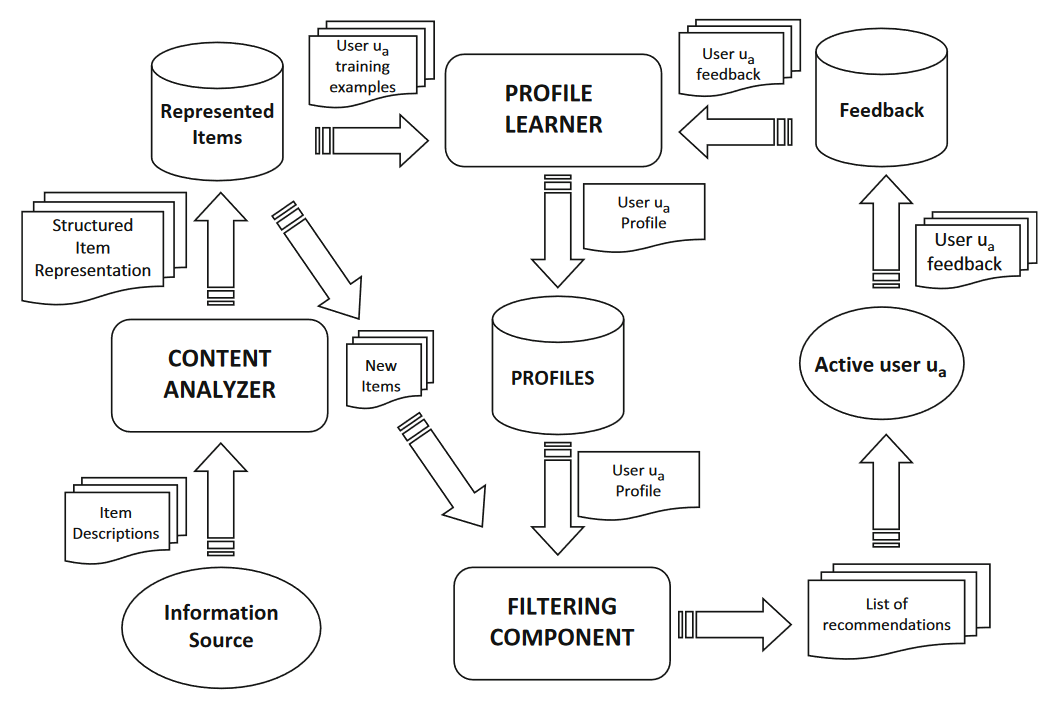
\includegraphics[width=0.9\textwidth]{img/content_based_figure_1.png}
    \caption{High level architecture of a content-based recommender \cite{Musto2022251}}
    \label{fig:high_lvl_content_based}
\end{figure}

The user modeling process has the goal to identify what are the users needs and this can be done 2 ways. Either the system calculates them from the interactions between the user and items through feedback or the user can specify these needs directly by giving keywords to the system, providing search queries \cite{Beel2016305}. \\\\
%
%
\textbf{Feedback}\\
When trying to acquire helpful information or criticism that is given by the user there are 2 separate ways. \\
The first one is called Explicit Feedback where it is necessary for the user to give item evaluation or actively rate products. Most popular options are gathering like/dislike ratings on items or the ratings can be on a scale either from 1 to 5 or 1 to 10. After the ratings the user can also give comments on separate items. \\\\
The other way is called Implicit Feedback where the information is collected passively from analyzing the users activities. Some alternatives can be clicks on products, time spent on sites or even transaction history \cite{DeGemmis2015119}.\\\\
%
%
%
\textbf{Advantages and Disadvantages of CB Filtering}
\begin{itemize}
\item User Idependence - meaning the ratings taken into consideration are only provided by the active user to build their own profile. Collaborative approaches will recommend items based on ratings from other users in the nearest neighborhood.
\item Transparency - explanations for the recommended items can be provided explicitly by listing the content features which were used to get that recommendation. On the other hand Collaborative systems are considered black boxes, where explanations are based on similar tastes of different users.
\item New Item - when a new item is added to the system, the Content-based method is capable of recommending it from the set features and its content. This is not possible for the Collaborative method which needs ratings for the new item to be able to recommend it.
\item Limited Content Analysis - because the system can only analyze a certain number of features and can miss important aspects such as aesthetics or other multimedia information. Also, systems based on string matching approach can suffer from problems such as synonymy, polysemy or multi-word expressions.
\item Over-Specialization - the user will mostly be recommended things similar to what they already liked, which drawback is called 'lack of serendipity'. For example, if the user only rated action movies, then the system would not recommend other genres, which limits the chance of recommending items with novelty or surpise. \cite{DeGemmis2015119}\\
\end{itemize}
%
%
%
%
\textbf{Semantic approaches in CB Recommendation}\\
In short Semantics refer to interpretation of meaning in language, words and symbols. Using semantic techniques the represantations of items and user profiles shift from keyword-based to concept-based ones.  With these represantations it is possible to give meaning to information expressed in natural language and to get a deeper understanding of the information presented by textual content.\\
Content-based recommendations can adopt two different approaches based on how the semantics are derived and applied:
\begin{itemize}
\item \textbf{Top-Down Semantic Approaches} use an external knowledge to improve the representation of the items and users. This external knowledge can be: ontological resources, encyclopedic knowledge (ESA, BabelNet) and the Linked Open Data cloud. For example the \textbf{Ontology} is a structured description that shows how different parts of a system depend on each other and how they are connected. It organizes key concepts in a specific domain into a hierarchy, which can explain their relationships and the characteristics of each concept. It can help to understand how specific examples of these concepts behave and how they are related \cite{pub.1090632691}.
%
\item \textbf{Bottom-Up Semantic Approaches} use implicit semantic representation of items and user profiles, where the meanings of terms are assumed by analyzing its usage. They rely on the distributional hypothesis: "words that occur in the same context tend to have similar meanings". Without a predefined structure, this approach analyzes the words co-occurrence with other words, larger texts or documents using Discriminative Models.\cite{DeGemmis2015119}\\
\end{itemize}
%
%
The semantic approaches can be further categorized by the source of knowledge used to extract meaning, which are \textbf{Endogenous Semantics} and \textbf{Exogenous Semantics}.\\
In the first case, the semantics is obtained by exploiting unstructured data, and is directly inferred from the available information. Different techniques for these Implicit Semantics Representations are for example the Term Frequency - Inverse Document Frequency (TF-IDF) weighting, or the Distributional Semantics Models (DSM) such as Explicit Semantics Analysis (ESA), Random Indexing or Word Embedding Techniques.
Word embedding technology can reflect the semantic information of words to a certain extent. The semantic distance between words can be calculated by word vectors. Commonly used word vectors are based on Word2vec and Fasttext models \cite{Huang2023}.\\\\
%
In the second, the semantics comes from the outside, since it is obtained by mining and exploiting data
which are previously encoded in structured and external knowledge sources. For these Explicit Semantics Representations there are also different techniques like Linking Item Features to Concepts using Word Sense Disambiguation (WSD) or using Entity Linking, or Linking Items to Knowledge Graphs using Ontologies or Linked Open Data (LOD). \cite{Musto2022251} \\
The LOD cloud is a huge decentralized knowledge base where researchers and organizations publish their data in Resource Description Framework (RDF) format and adopt shared vocabularies, in order to express an agreed semantics and interlink the data to each other \cite{Musto2017405}.\\
%
%
%
%\clearpage
\subsubsection{Knowledge Graphs}
Knowledge graph is a knowledge base that uses a graph-structured data model. It is a graphical databases which contains a large amount of relationship information between entities and can be used as a convenient way to enrich users and items information \cite{Imene2022488}.\\
%
The idea is that attributes of users and items are not isolated but linked up with each other, which forms a knowledge graph (KG). Incorporating a Knowledge Graph into recommendations can help the results in ways like:
\begin{itemize}
\item The rich semantic relatedness among items in a KG can help explore their latent connections and improve the precision of results
\item The various types of relations in a KG are helpful for extending a user’s interests reasonably and increasing the diversity of recommended items
\item KG connects a user’s historically-liked and recommended items, thereby bringing explainability to recommender systems. \cite{Wang20193307}
\end{itemize}
%
Basically a knowledge graph is a directed graph whose nodes are the entities and the edges are the relations between them. They are usually defined as triplets with a head entity, tail entity and a relationship connecting them. The graphs have detailed supporting information which is background knowledge of items and their relations amongst them. The facts of items are organized in those triplets like (Ed Sheeran, IsSingerOf, Shape of You), which can be seamlessly integrated with user-item interactions. This interaction data is usually presented as a
bipartite graph \cite{pub.1120733877}. \\
The crucial point to leverage knowledge graphs to perform item recommendations is to be able to effectively model user-item relatedness from this rich heterogeneous network \cite{Palumbo201732}. \\\\ 
%
%
%
Recommendation methods based on knowledge graphs can be practically categorized into two different types which are Path-based and Embedding-based methods. Where the \textbf{Embedding-based} method uses knowledge graph embedding (KGE) techniques trying to learn how to represent users and items. This method uses representation learning to find connections implicitly, rather than using user preferences. Models such as TransE, TransR and TransH build entity and relation embeddings by regarding a relation as translation from head entity to tail entity. These models simply put both entities and relations within the same semantic space. \cite{pub.1148917041}\\
The \textbf{Path-based} method focuses on enhancing the connections called meta-paths that link the users and items, showing how similar they are \cite{Yang20229308}. \\
%


\subsubsection{Hybrid Approaches}
The Hybrid recommender systems try to combine two or more recommendation techniques to get to better performance and accuracy. The most common approach is to have a collaborative filtering technique combined with some other technique to try to avoid the ramp-up problem.
The ramp-up problem actually means two problems, which are "New User" and "New Item" problems (hard to categorize with few ratings).\\
Different types of hybrid recommender systems exist, which are the following \cite{Burke2002331}:
\begin{itemize}[label=--]
\item \textbf{Weighted hybrid} - initially gives equal weight to all available recommendation techniques in the system. Gradually adjusts the weighting based on wether the predicted user ratings are confirmed or discomfirmed. The recommended items score is computed from the results.
\item \textbf{Switching hybrid} - the system switches between recommendation techniques based on some criterion. The advantage is that the system can adapt to the strengths and weaknesses of the different recommendation methods it combines.
\item \textbf{Mixed hybrid} - recommendations from more than one technique are presented together at the same time. 
\item \textbf{Feature combination} - for example in a content / collaborative merger the system treats the collaborative information as an additional feature data and uses content-based techniques over this enhanced dataset.
\item \textbf{Cascade hybrid} - one recommender produces a coarse ranking of candidates and than the other refines the recommendations given by the first one. The second step only focuses on the items given by the first step and not all items in the dataset.
\item \textbf{Feature augmentation} - one technique produces a rating of an item and that information is then incorporated into processing the next recommendation technique. The features used by the second recommender include the output of the first one (like ratings).
\item \textbf{Meta-level hybrid} - combines two techniques by using the model generated by one as the input for the other, meaning the entire model becomes the input.\\
\end{itemize}
%
%
%
%%%%%%%%%%%%%%%%%%%%%%%%%%%%%%%%%%%%%%%%%%%%%%
%
\subsection{Difficulties related to Recommendation Systems}
All types of recommendation systems encounter significant challenges which they have to face and issues they have to solve. Here are some main challenges:
%
\begin{itemize}
\item Cold-start problem - arises when making recommendations to new users and/or items for which the available information is limited. As a result, the recommendations offered in such cases tend to be of poor quality and lack usefulness.\cite{Al-Hassan2024a}
\item Data sparsity - when recommender systems use large datasets, the user-item matrix used for filtering can be sparse, which leads to worse performance of recommendations.
\item Scalability - as the number of users and items increases, so does the complexity of the algorithms used for recommending items.
\item Diversity - helps to discover new products, but some algorithms may accidentally do the opposite, which can also lead to lower accuracy in the recommendation process. \cite{pub.1072601078}
\item Privacy - because the information collected by the system usually includes sensitive information that users wish to keep private, users may have a negative impression if the system knows too much about them.
\item Serendipity - sometimes can be useful, but if the result of the recommendation system only has
serendipitous items and does not have related items, user may think that the system is not reliable. \cite{Aymen2022896}\\
%\item Exploration vs. Exploitation
\end{itemize}


%%%%%%%%%%%%%%%%%%%%%%%%%%%%%%%%%%%%%%%%%%%%%%

\subsection{Evaluation of Recommendation Systems}
When trying to choose which recommendation approach is the best, first it is important to know the use case for the specific system. \\
The process of finding the most appropriate algorithm for the specific goal typically is based on experiments, comparing the performance of a number of candidate recommenders. Comparing the performance of an algorithm is mostly performed by using some evaluation metric, which usually uses numeric scores, that provides ranking of the compared algorithms. \\
For measuring the accuracy of predictions of the algorithm three classes of measurements are defined, which are \cite{Gunawardana2022547}:
\begin{itemize}
\item \textbf{Measuring Ratings Prediction Accuracy} wishes to measure the accuracy of the system's predicted ratings. The following metrics can be used in such situation: Root Mean Squared Error (RMSE), Mean Absolute Error (MAE), Normalized RMSE, Normalized MAE, Average RMSE, Average MAE.
\item \textbf{Measuring Usage Prediction} tries to recommend to users items that they may use, with the following metrics: Precision, Recall (True Positive Rate), False Positive Rate (1 - Specificity), F-measure, Area Under the ROC Curve (AUC).
\item \textbf{Ranking Measures} is not predicting an explicit rating, but rather is ordering items according to the user's preferences. This can be done Using a Reference Ranking like Normalized Distance based Performance Measure (NDPM), Average Precision (AP) correlation, Spearman's rank correlation coefficient, Kendall's rank correlation coefficient or using Utility-Based Ranking such as Normalized Discounted Cumulative Gain (NDCG), Discounted Cumulative Gain (DCG) or Average Reciprocal Hit Rank (ARHR). Other than that there is also Online Evaluation of Ranking.
\end{itemize}
%
%
%
However, not all users are trying to use the recommendation engine just for the most accurate predictions, but they might be more interested in other properties of the recommender system like \cite{Gunawardana2022547}:
\begin{multicols}{3}
\begin{itemize}
\item Coverage
\item Confidence
\item Trust
\item Novelty
\item Serendipity
\item Diversity
\item Utility
\item Risk
\item Robustness
\item Privacy
\item Adaptability
\item Scalability
\end{itemize}
\end{multicols}
%
%
%
In the domain of scientific publications, where users are relatively few with respect to the available documents, information needs and interests easily change in an unpredictable way over time due to evolving professional needs, there is no advertising pushing new items, and the long tail of infrequently read articles may contain the so-called sleeping beauties, that are documents containing extremely relevant results, but that remain unknown to most researchers for a very long time. \\
The Content-based approach does not require particular assumptions over the size and the activity of the user base. It does not penalize items that have less ratings or are less frequently consumed by many users as long as enough metadata are available, which even allows detailed explanations. These advantages over Collaborative Filtering techniques make this approach particularly attractive to the purpose of providing recommendation in the domain of scientific publications \cite{De_Nart201484}. \\
%
A study shows that more than half of the recommendation approaches applied Content-based filtering, when making recommendations for research papers and articles in libraries \cite{Beel2016305}. \\
%





%%%%%%%%%%%%%%%%%%%%%%%%%%%%%%%%%%%%%%%%%%%%%%%%%%%
%\begin{itemize}
%\item 
%\item 
%\end{itemize}


\clearpage
\section{Implementation Proposal}
% 5-10 Pages \\\\
When evaluating a RS there are two main types of evaluation, which are:
\begin{itemize}
\item System-Centric Evaluation
	\begin{itemize}
	\item Algorithmic Aspects - e.g., the predictive accuracy of recommendation algorithms
	\end{itemize}

\item User-Centric Evaluation
	\begin{itemize}
	\item Users' Perspective - how users perceive its quality or the user experience when interacting with the RS
	\end{itemize}

\end{itemize}

\subsection{Experiment Types}
\begin{table}[h!]
\centering
\begin{tabular}{p{3cm}|p{10cm}}
\hline
\textbf{Type} & \textbf{Description} \\
\hline
Offline & Method: simulation of user behavior based on past interactions \\
        & Task: defined by the researcher, purely algorithmic \\
        & Repeatability: evaluation of an arbitrary number of experiments possible at low cost \\
        & Scale: large dataset, large number of users \\
        & Insights: quantitative, narrow \\
\hline
User Study & Method: user observation in live or laboratory setting \\
           & Task: defined by the researcher, carried out by the user \\
           & Repeatability: expensive \\
           & Scale: small cohort of users \\
           & Insights: quantitative and/or qualitative \\
\hline
Online & Method: real-world user observation, online field experiment \\
       & Task: self-selected by the user, carried out by the user \\
       & Repeatability: expensive \\
       & Scale: large \\
       & Insights: quantitative and/or qualitative \\
\hline
\end{tabular}
\caption{Overview of Experiment Types \cite{Zangerle2023}}
\end{table}
%
%
\textbf{Offline evaluations} are the most popular experiment type. They aim to compare different recommendation algorithms and settings; they do not require any user interaction and may be considered
system-centric.  \cite{Zangerle2023}\\\\
%
%
Choices:
\begin{itemize}
\item different datasets
\item different evaluation goals
\item different metrics to compare
\end{itemize}
%
%
%
\begin{figure}[h!]
    \centering
    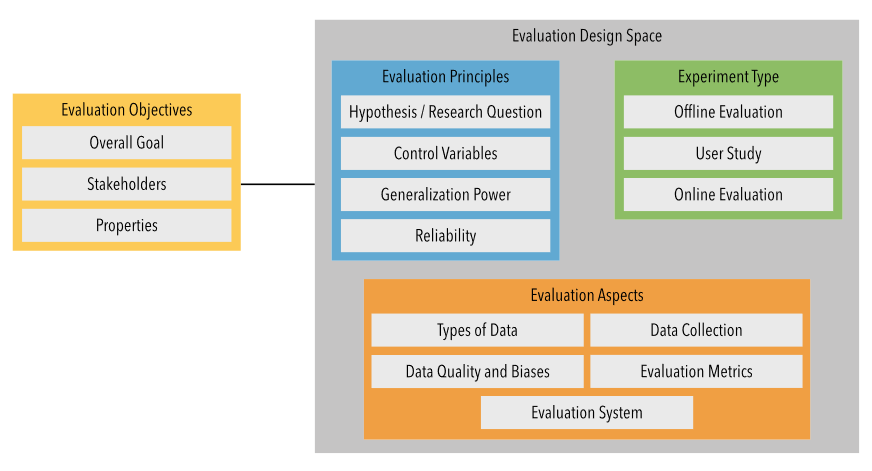
\includegraphics[width=0.9\textwidth]{img/evaluation_figure.png}
    \caption{Evaluation of Recommender Systems: objectives and design space \cite{Zangerle2023}}
    \label{fig:evaluation}
\end{figure}
%
%
%
\textbf{Evaluation Objectives} ~\ref{fig:evaluation}.
%
\begin{itemize}
\item Overall Goal - importance to define the evaluation goal as precisely as possible
\item Stakeholders - varying goals and potentially conflicting interests\\
Currently, academic RS research tends to take the perspective of the end consumer
\item Properties - improving specific properties where they fall short \\
The challenge is to identify the properties that are indeed relevant for a recommender’s performance and show that it affects the users’ experience, or the interests of other stakeholders. 
\end{itemize}
%
%
%
\textbf{Evaluation Design Space:\\ Evaluation Principles} ~\ref{fig:evaluation}.
%
\begin{itemize}
\item Hypothesis - precisely define the evaluation’s goal - the more precise the hypothesis, the clearer
the evaluation setup as the hypothesis (in line with the evaluation objectives) shapes the evaluation design
“Our recommendation algorithm based on visual features leads to a higher recommendation accuracy in comparison with conventional genre-based recommender systems” 

\item Research Question -  when little is known about the phenomenon. The problem cannot be clearly defined at this state of research and the evaluation might, be of exploratory nature - to get a better understanding of a problem or explore patterns

\item Control Variables
\item Generalization Power
\item Reliability
	\begin{itemize}
	\item Reproducibility (different team, different experimental setup)
	\item Repeatability (same team, same experimental setup)
	\item Replicability (different team, same experimental setup)
	\end{itemize}
\end{itemize}
%
%
%
\textbf{Evaluation Aspects} ~\ref{fig:evaluation}.
%
\begin{itemize}
\item Types of Data
	\begin{itemize}
	\item Implicit and Explicit Rating Data
	\item User, Item Information
	\item Qualitative and Quantitative Data
	\item Natural and Synthetic Data
	\end{itemize}
\item Data Collection
	\begin{itemize}
	\item User Involvement
	\item User Feedback Elicitation
	\item Existing Datasets
	\end{itemize}
\item Data Quality and Biases
\item Evaluation Metrics
\item Evaluation System
\end{itemize}
%
%
%
%
%
\begin{table}[h!]
\centering
\caption{FEVR: Overview of Example Evaluation}
\begin{tabular}{lp{10cm}}
\hline
\textbf{FEVR Component} & \textbf{Brief Description} \\ \hline
\multicolumn{2}{|l|}{\textbf{Evaluation Objectives}} \\ \hline
Overall Goal & To evaluate whether users are able to find likable music in the recommendations computed by the novel RecAlg algorithm \\ \hline
Stakeholders & Users of the system (algorithm) \newline Artists may also benefit from an increased item diversity as a more diverse set of artists may be represented \\ \hline
Properties & Item diversity in the recommendations; catalog coverage \\ \hline
\multicolumn{2}{|l|}{\textbf{Evaluation Principles}} \\ \hline
Hypothesis/Research Question & \( H_1 \): RecAlg provides users (on average) with more diverse recommendations with respect to the intra-list diversity while maintaining prediction accuracy compared to the baseline algorithm. \\ \hline
Control Variables & Follow accountability framework by Bellogín and Said \cite{24} (for randomization in dataset splitting to prevent selection bias) \\ \hline
Generalization Power & Limited due to lack of user involvement and dataset biases \\ \hline
Reliability & Follow accountability framework by Bellogín and Said \cite{24} \\ \hline
\multicolumn{2}{|l|}{\textbf{Experiment Type}} \\ \hline
Experiment Type & Offline Evaluation with A/B-testing \\ \hline
\multicolumn{2}{|l|}{\textbf{Evaluation Aspects}} \\ \hline
Types of Data & Implicit ratings (listening events), side information for music tracks \\ \hline
Data Collection & LFM-2b dataset \cite{194} \\ \hline
Data Quality and Biases & Platform bias, popularity bias, skewed gender distribution, imbalanced country distribution \\ \hline
Evaluation Metrics & Prediction accuracy with RMSE; intra-list similarity in terms of different unique artists \\ \hline
Evaluation System & Existing evaluation framework Elliot \cite{14} \\ \hline
\end{tabular}
\end{table}
%
%


\clearpage
\textbf{METRICS TO USE}:
\begin{itemize}
\item Relevance - Feature Similarity

\item Accuracy -> NEEDS RATINGS
\item Usage Prediction -> NEEDS IMPLICIT FEEDBACK (clicks, downloads...)

\item Ranking Measure
\item Diversity
\item Novelty - maybe (Serendipity is almost the same)
\item Confidence\\\\
\end{itemize}



\textbf{TASK 1:} Recommend books (list of books) based on 1 book (opened book)\\\\
\textbf{TASK 2:} Recommend books (list of books) based on users query (the querys meaning - content) (not like a search engine)\\









\clearpage
\thispagestyle{empty}
\mbox{}



%%%%%%%%%%%%%%%%%%%%%%%%%%%%%%%%%%%%%%%%%%%%%%%%%%%

\clearpage{}
\section{Implementation}
5 Pages\\\\

\subsection{Dataset}

\subsection{Experiments}
\cite{Gunawardana2022547}
%
\begin{itemize}
\item Offline Experiments - performed by using a pre-collected data set of users choosing or rating items
\item User Studies - real user interaction with the system is collected, questions are asked (how relevant were the recommendations …)
\item Online Evaluation - the system is used by real users that perform real tasks. It is most trustworthy to compare a few systems online, obtaining a ranking of alternatives, rather than absolute numbers that are more difficult to interpret.
\end{itemize}

\subsection{Testing}
\cite{Gunawardana2022547}
%
\begin{itemize}
\item Confidence and p-values
\item Paired Results - sign test, McNemar's test, paired Student's t-test, Wilcoxon signed rank test
\item Unpaired Results - Mann-Whitney test
\item Multiple Tests - ANOVA, Friedman test for ranking
\item Confidence Intervals - Gaussian distribution, mean, standard dev
\end{itemize}
%

%%%%%%%%%%%%%%%%%%%%%%%%%%%%%%%%%%%%%%%%%%%%%%%%%%%

\clearpage{}
\section{Conclusion}
3-4 Pages\\\\



\clearpage
\thispagestyle{empty}
\mbox{}






%%%%%%%%%%%%%%%%%%%%%%%%%%%%%%%%%%%%%%%%%%%%%%%%%%%

\clearpage 
\normalsize 
\bibliographystyle{unsrt} 
\bibliography{literature} 
\nocite{*}

\end{document}
